\documentclass[12pt, oneside]{book}
\usepackage[a4paper,top=2.5cm,bottom=2.5cm,left=3.5cm,right=2cm,footskip=.25in]{geometry}
\usepackage[utf8]{inputenc}
\usepackage[T1]{fontenc}
\usepackage{graphicx}
\usepackage{url}
\usepackage{float}
\usepackage{mathtools}
\usepackage{amsmath}
\usepackage{amssymb}
\usepackage{lmodern}
\usepackage{indentfirst}
\usepackage{enumerate}
\usepackage{array}
\usepackage{ragged2e}
\usepackage{lipsum}
\usepackage{array}
\usepackage{subcaption}
\usepackage{hyperref}

\usepackage{listings}
\usepackage{color}

\definecolor{dkgreen}{rgb}{0,0.6,0}
\definecolor{gray}{rgb}{0.5,0.5,0.5}
\definecolor{mauve}{rgb}{0.58,0,0.82}




\usepackage[
backend=bibtex
% backend=biber % <-- biber is a modern replacement for BibTeX designed for use (only) with biblatex
]
{biblatex}
\addbibresource{bibliography.bib}

\usepackage{hyperref}
\hypersetup{
    colorlinks,
    citecolor=black,
    filecolor=black,
    linkcolor=black,
    urlcolor=black
}

\usepackage[slovak]{babel}
%\renewcommand{\baselinestretch}{1.8} 

% toto som zmenil aby som mal viac textu na seminar :D
\linespread{1.25} % hodnota 1.25 by mala zodpovedat 1.5 riadkovaniu

% -------------------
% --- Definicia zakladnych pojmov
% --- Vyplnte podla vasho zadania
% -------------------
\def\mfrok{2019}
\def\mfnazov{Porovnanie niekoľkých typov rekurentných sietí z hľadiska hĺbky pamäte}
\def\mftyp{Diplomová práca}
\def\mfautor{Bc. Jaroslav Ištok}
\def\mfskolitel{doc. RNDr. Martin Takáč, PhD.}


%ak mate konzultanta, odkomentujte aj jeho meno na titulnom liste
%\def\mfkonzultant{ }  

\def\mfmiesto{Bratislava, \mfrok}

%aj cislo odboru je povinne a je podla studijneho odboru autora prace
\def\mfodbor{2511  Aplikovaná informatika} 
\def\program{ Aplikovaná informatika }
\def\mfpracovisko{ Katedra aplikovanej informatiky }

\begin{document}     

% -------------------
% --- Obalka ------
% -------------------
\thispagestyle{empty}

\begin{center}
\sc\large
 Univerzita Komenského v Bratislave\\
 Fakulta matematiky, fyziky a informatiky
\vfill

{\LARGE\mfnazov}\\
\mftyp

\end{center}

\vfill

{\sc\large 
\noindent \mfrok\\
\mfautor
}

\eject % EOP i
% --- koniec obalky ----

% -------------------
% --- Titulný list
% -------------------

\thispagestyle{empty}
\noindent
"" 
\begin{center}
\sc  
\large
 Univerzita Komenského v Bratislave\\
 Fakulta matematiky, fyziky a informatiky

\vfill

{\LARGE\mfnazov}\\
\mftyp
\end{center}

\vfill

\noindent
\begin{tabular}{ll}
Študijný program: & \program \\
Študijný odbor: & \mfodbor \\
Školiace pracovisko: & \mfpracovisko \\
Školiteľ: & \mfskolitel \\
% Konzultant: & \mfkonzultant \\
\end{tabular}


\vfill


\noindent \mfmiesto\\
\mfautor

\eject % EOP i


% --- Koniec titulnej strany


% -------------------
% --- Zadanie z AIS
% -------------------
% v tlačenej verzii s podpismi zainteresovaných osôb.
% v elektronickej verzii sa zverejňuje zadanie bez podpisov

\newpage 
\thispagestyle{empty}
\hspace{-2cm}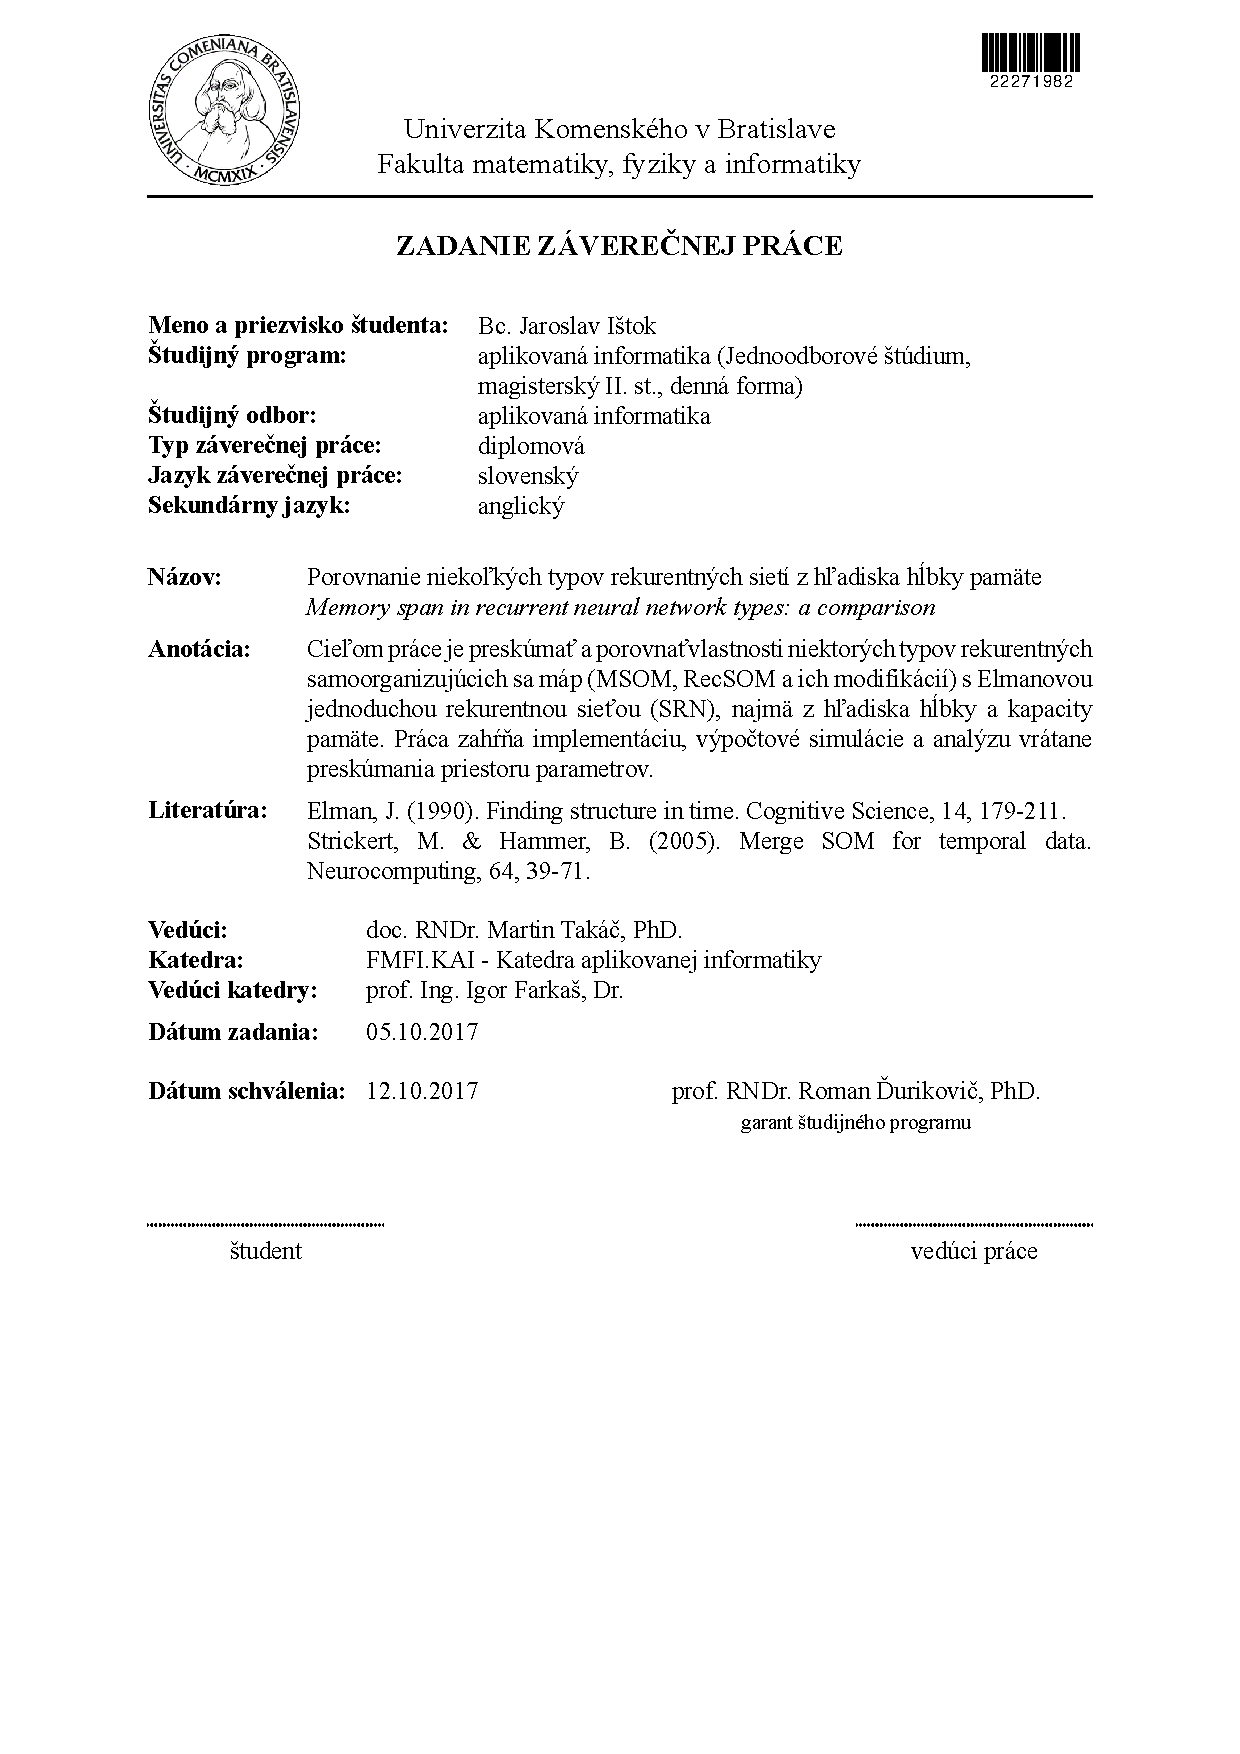
\includegraphics[width=1.1\textwidth]{assets/zadanie_master_thesis}


% --- Koniec zadania

\frontmatter

% -------------------
%   Čestné výhlásenie 
% -------------------
\setcounter{page}{3}
\newpage 
~
\vfill
{\bf Čestné vyhlásenie: Čestne prehlasujem, že som túto diplomovú prácu vypracoval samostatne len s použitím uvedenej literatúry a za pomoci môjho školiteľa diplomovej práce.}

% --- Koniec čestného  výhlásenia



% -------------------
%   Poďakovanie - nepovinné
% -------------------
 \setcounter{page}{3}
 \newpage 

 ~

 \vfill
 {\bf Poďakovanie: Chcel by som poďakovať svojmu školiteľovi, doc. RNDr. Martin Takáčovi, PhD., za jeho 
 pomoc, dlhé hodiny konzultácii, poskytnuté materiály a hlavne za usmernenie správnym smerom. }


% --- Koniec poďakovania


% -------------------
%   Abstrakt - Slovensky
% -------------------
\newpage 
\section*{Abstrakt}
Použitie rekurentných neurónových sietí na spracovanie
sekvenčných dát je čoraz viac dôležité v dnešnej dobe v oblasti neurónových sietí.
V našej práci implementujeme niekoľko typov neurónových sietí a porovnávame ich z hľadiska hĺbky pamäte.
Hľadáme optimálne parametre, pri ktorých majú rôzne typy neurónových sietí najvyššie hodnoty pamäťových hĺbok.
Získané výsledky následne porovnávame a analyzujeme súvislosti medzi hodnotami parametrov a pamäťovou hĺbkou siete. 
Následne analyzujeme a porovnávame výsledky pre testované typy sietí.

\paragraph*{Kľúčové slová:} rekurentné neurónové siete, hĺbka pamäte, samorganizujúca sa mapa
% --- Koniec Abstrakt - Slovensky


% -------------------
% --- Abstrakt - Anglicky 
% -------------------
\newpage 
\section*{Abstract}
Usage of recurrent neural nets for processing sequential data is getting more important nowadays in the area of neural networks.
In our work we implement several types of neural nets which we compare in terms of their memory span.
We find optimal parameters for which different types of tested neural nets have the highest memory span values.
Then we analyze the results and compare them for tested neural nets.


\paragraph*{Keywords:} neural net, machine learning, memory span, self organizing map

% --- Koniec Abstrakt - Anglicky

% -------------------
% --- Predhovor - v informatike sa zvacsa nepouziva
% -------------------
%\newpage 
%\thispagestyle{empty}
%
%\huge{Predhovor}
%\normalsize
%\newline
%Predhovor je všeobecná informácia o práci, obsahuje hlavnú charakteristiku práce 
%a okolnosti jej vzniku. Autor zdôvodní výber témy, stručne informuje o cieľoch 
%a význame práce, spomenie domáci a zahraničný kontext, komu je práca určená, 
%použité metódy, stav poznania; autor stručne charakterizuje svoj prístup a svoje 
%hľadisko. 
%
% --- Koniec Predhovor


% -------------------
% --- Obsah
% -------------------

\newpage 

\tableofcontents

% ---  Koniec Obsahu

% -------------------
% --- Zoznamy tabuliek, obrázkov - nepovinne
% -------------------

\newpage 

\listoffigures

\listoftables

% ---  Koniec Zoznamov

\mainmatter


\input uvod.tex 
\input podobne_prace.tex
\input navrh_riesenia.tex
\input implementacia.tex
\input experiment.tex
\input zaver.tex

% -------------------
% --- Bibliografia
% -------------------


 \addcontentsline{toc}{chapter}{Bibliography}
\newpage	

\backmatter

\thispagestyle{empty}
\nocite{*}
\clearpage

\printbibliography

% -------------------
%--- Prilohy---
% -------------------

%Nepovinná časť prílohy obsahuje materiály, ktoré neboli zaradené priamo  do textu. Každá príloha sa začína na novej strane.
%Zoznam príloh je súčasťou obsahu.
%
%\addcontentsline{toc}{chapter}{Appendix A}
%\input AppendixA.tex
%
%\addcontentsline{toc}{chapter}{Appendix B}
%\input AppendixB.tex

\end{document}






